% SPDX-FileCopyrightText: © 2026 Idiap Research Institute <contact@idiap.ch>
%
% SPDX-FileContributor: Andre Freitas <andre.freitas@idiap.ch>
% Neuro-symbolic AI Group
%
% SPDX-FileContributor: Danilo Gusicuma <danilo.gusicuma@idiap.ch>
% Neuro-symbolic AI Group
%
% SPDX-License-Identifier: MIT
\section{Manage recursive goals without losing the conceptual question}
\label{sec:recursive-goals}
A conceptual transformation changes what needs to be understood next. Replacing
coordinate identity by observable identity creates a question about compatible
dynamics; answering that question can require a lemma about equivalence classes,
a calculation, or a counterexample. Recursion arises when a task exposes a
smaller unresolved question that needs its own investigation. It also arises
when a failed subsidiary calculation reveals that the parent question must change.
The organizing principle is to preserve the reason for pursuing each child while
allowing its result to revise that reason.

The repository's formal-subgoal policy requires a target object, preserved
commitments, current blocker, learning from the last failure, next action and
conditions for changing or stopping the route. Its cumulative result atlas
separates durable scientific results from the next-action queue. The completed
subgoal auditor separately asks what a local achievement actually enables.
The following account synthesizes those prescriptions into a management model;
it is not a claim that the nineteen native declarations implement one recursive
scheduler.\footnote{\raggedright Sources: \path{docs/research-methods/formal-subgoal-control-policy.md},
\path{docs/research-methods/result-subgoal-atlas.md}, and
\path{skills/evaluation/completed-subgoal-enablement-auditor/SKILL.md}.}

\subsection{Give each goal an identity and an acceptance condition}
Use a short record that separates the question from its inputs and result:
\begin{description}[style=nextline,leftmargin=1.7cm,labelwidth=1.5cm,itemsep=1pt,parsep=0pt,topsep=4pt]
\item[Goal] Exact question, identifier/version, parent requirement and dependencies.
\item[Input] Target, carrier, representation, assumptions, evidence and open obligations.
\item[Accept] Evidence required for this question at its stated scope.
\item[Output] Scoped result or failure, supporting evidence and remaining debt.
\item[Next] Bounded attempt or handoff; stopping and reopening conditions.
\end{description}
A label such as ``prove descent'' does not preserve context: linear and nonlinear
dynamics define different questions. Record a new version or explicit replacement
when the claim changes.

Acceptance depends on the kind of goal. A proof goal needs a valid argument
for the exact statement and assumptions. A conceptual goal may instead ask for
an articulated alternative that preserves specified successes and exposes a
consequential new question. Satisfying the latter closes that articulation task;
it does not establish the alternative as true or close its ensuing proof debt.
The acceptance condition must remain visible when the task is delegated, so
that an attractive easier result cannot silently replace the intended answer.

An attempt is a bounded action on a goal: try a lemma, reconstruct an objection,
search for a source, or compare two representations. Several attempts can address
the same goal. Finishing or cancelling an attempt does not in itself settle the
goal. Conversely, a certified result may settle a precise child while its parent
remains unresolved. This separation permits honest stopping without deleting
useful work or overstating what has been achieved.

\subsection{Decompose obligations and alternatives differently}
Two relationships must be kept distinct. In a \emph{conjunctive} decomposition,
all specified children are required: a quotient dynamics may need both
representative independence and the relevant solution existence conditions.
The parent can close only when those child results are accepted in compatible
contexts and their composition actually establishes its criterion. Completing
one required child leaves the other obligation open.

In an \emph{alternative-route} decomposition, children explore different ways
to answer the same parent question. One route can suffice if it meets the
parent's full acceptance condition. Failure of another route does not defeat
that answer, and failure of every route tried does not establish that all
possible routes are impossible. Moreover, a comparison goal can require several
alternatives to be examined before any preference is justified. Calling its
branches ``alternatives'' does not license closing that comparative task after
the first favorable result.

The result is a dependency graph, even when delegation is displayed as a tree.
A lemma or conceptual objection can serve several parents. Reuse requires the
same statement, assumptions and relevant object identity, or a justified
translation between them. Shared results retain separate acceptance decisions
for their consumers. An ancestor cannot be certified by a descendant that
assumes the very claim under investigation; such a circular dependency remains
an open obligation unless a separate legitimate mathematical principle discharges
it. Revisiting an earlier question is instead represented by a new attempt or
version with an explicit change, not by counting a cycle as new evidence.

\begin{figure}[htbp]
\centering
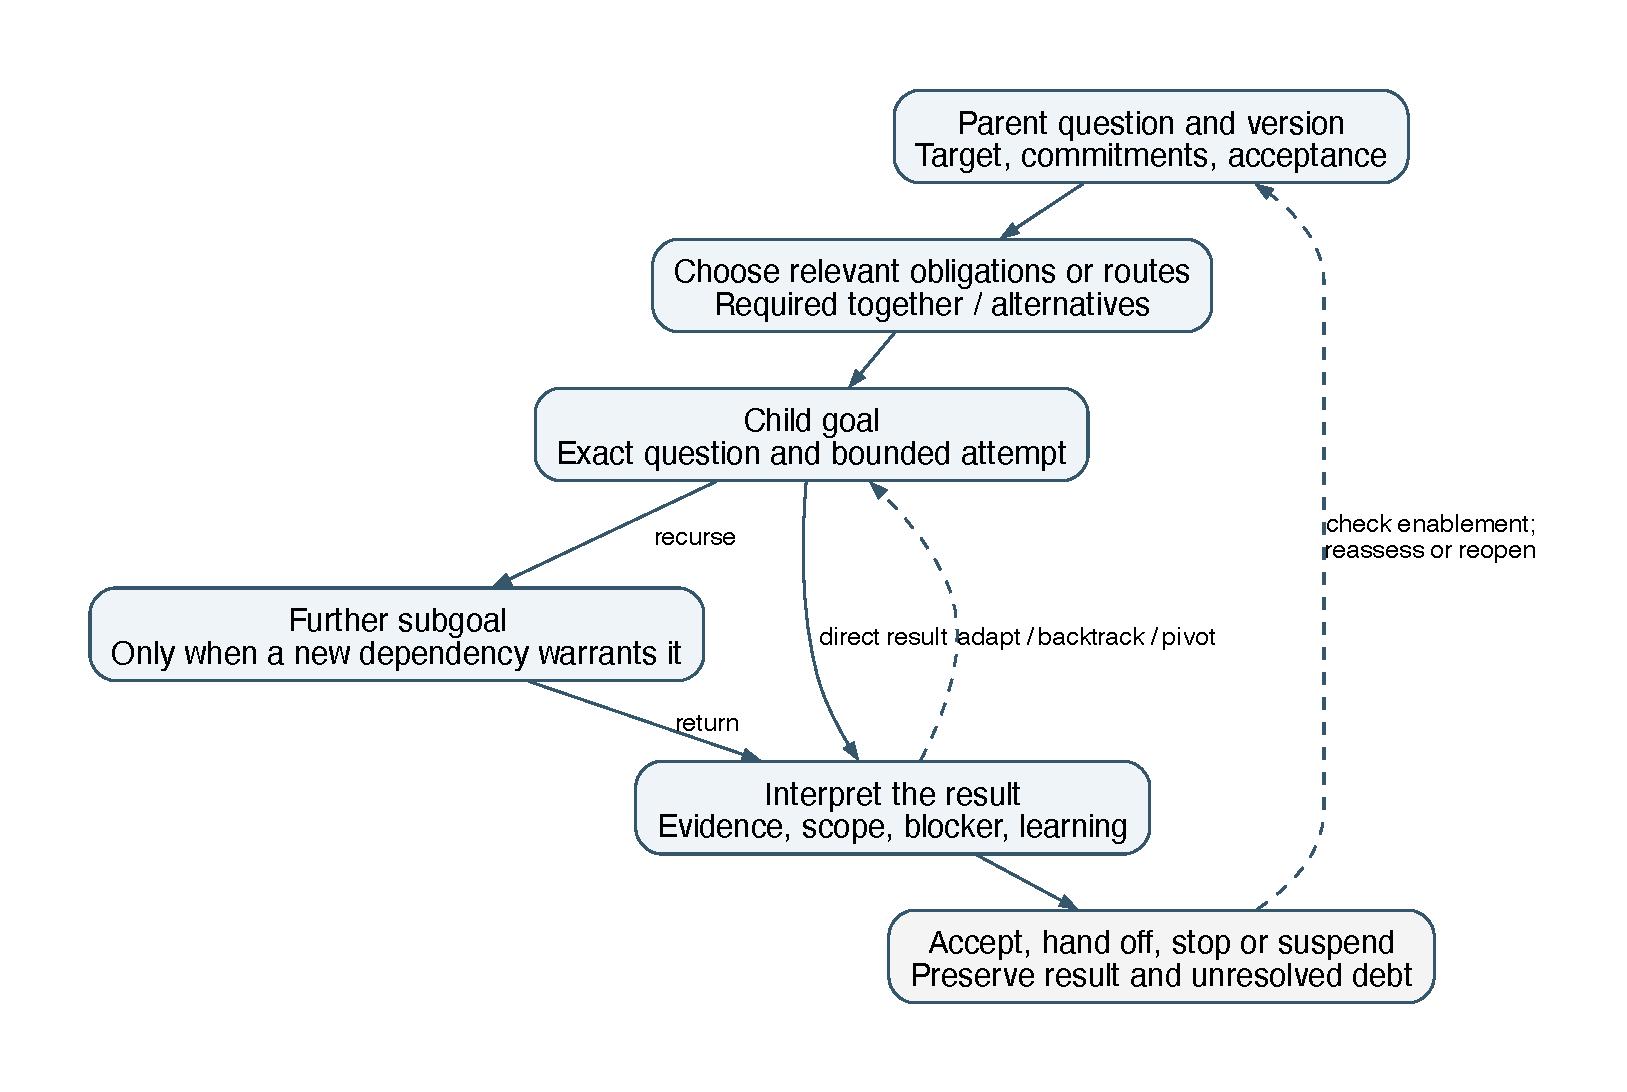
\includegraphics[width=.94\linewidth]{paper-workflow-representations/recursive-goals.pdf}
\caption{Recursive investigation as accountable decomposition and return.
The arrows express the management model in the text, not a recovered runtime
call graph. A child's report changes its parent's evidence and next decision;
it does not automatically mark that parent achieved.}
\label{fig:recursive-goals}
\end{figure}

\subsection{Decide whether to continue, change direction or stop}
A useful next attempt needs both a live connection to the target and a named
possible gain: discharge an obligation, discriminate alternatives, expose a
hidden premise, or make an explanation more precise. A failed attempt can justify
continuation when it supplies such information and changes the next move.
Repetition with unchanged inputs, the same blocker and no new learning needs a
control decision rather than another optimistic restatement.

\begin{table}[htbp]
\centering\small
\begin{tabularx}{\linewidth}{@{}>{\raggedright\arraybackslash}p{.17\linewidth}>{\raggedright\arraybackslash}X>{\raggedright\arraybackslash}X@{}}
\toprule
Decision & Criterion for the work & What returns to the parent \\
\midrule
Continue or adapt & Target remains relevant; the next bounded move has an explicit informative payoff & New attempt, changed formulation or discriminating check; goal remains open \\
Backtrack & An assumed premise, object identity or transfer has not been established & The missing prerequisite and the claims conditional on it \\
Pivot & The route repeatedly fails without useful new learning; a materially different route is justified & Preserved failure evidence and a new route, with no inherited proof status \\
Quarantine & Analogy, weaker scope or an unverified bridge prevents intended use & A retained result with restricted authority and conditions for rehabilitation \\
Stop or suspend & No target-relevant informative move is available, resources end, or a required dependency is unavailable & Terminal attempt or inactive branch; unresolved goal and reason remain recorded \\
Accept or hand off & The exact local acceptance criterion is met, or a bounded result is ready for its next validation stage & Scoped result, remaining debt and explicit parent-enablement check \\
\bottomrule
\end{tabularx}
\caption{An explanatory synthesis of source control distinctions. These are
work decisions, not a single scale of scientific confidence. Handoff and
resource exhaustion are especially distinct from proof.}
\label{tab:goal-stopping}
\end{table}

The stopping rule should be selected for the task rather than inferred from
how hard the problem feels. The contribution-oriented manager, for example,
prescribes at least two explicit adaptations or backtracks before stopping a
branch that still cannot name a contribution candidate, a disqualifying test or
a target-preserving validation handoff. This is a local contribution-search
policy, not a universal recursion depth or a guarantee that two attempts suffice.
The same source says not to stop solely because proof debt is hard. It also
requires broad exploration to end once a smallest defensible contribution has
reached its specified handoff boundary: validation and packaging then become
the appropriate work.\footnote{\path{skills/orchestration/contribution-oriented-subgoal-manager/SKILL.md},
``Good-Enough And Stop Policy.''}

Operational limits answer a different question: how much work may this attempt
consume? A recursion controller can allocate a finite total budget, cap depth
and live branches, charge children against the same budget, and require each
new expansion to identify what it adds. A stopped child must not acquire a
fresh unlimited allowance by being renamed or respawned. These are proposed
implementation disciplines for the explanatory model. Bounded expansion and
interruptible, bounded-duration actions can bound a run; a depth limit alone
cannot prevent unlimited sibling attempts, and none of these limits proves
scientific completeness or semantic convergence. Exhaustion returns ``unresolved
within this allocation,'' not ``false'' or ``impossible.''

\subsection{Return results, re-evaluate parents and reopen selectively}
The child returns a compact handoff:
\begin{description}[style=nextline,leftmargin=1.7cm,labelwidth=1.5cm,itemsep=1pt,parsep=0pt,topsep=4pt]
\item[Input] Exact parent requirement and goal version.
\item[Output] Result or failure; evidence, assumptions, scope and remaining debt.
\item[Check] Current context, required dependency and compatibility with sibling results.
\item[Next] Accept the supported contribution, revise the task or retain an unresolved obligation.
\end{description}
A lemma about the wrong carrier or a weaker quantifier can retain local value
without enabling parent closure.

If the parent changes its representation, premise or target, previously returned
children must be checked against that change. Some remain applicable, others
need translation or renewed work, and some become irrelevant to the revised
question. Historical results need not become false when their applicability
changes. Reopening follows the actual dependency chain: record the changed
assumption or evidence, the affected consumers, and a reason why renewed work
could now be informative. A late result for an old version is preserved and
reassessed; it is not silently attached to the current parent. Stopped or
quarantined branches can likewise reopen when a missing bridge, new source,
changed commitment or justified new allocation changes the decision conditions.
Renewed resources can resume unresolved work; they cannot rehabilitate a refuted
claim under unchanged assumptions. That requires a revised claim or context, or
evidence that defeats the purported counterexample.

\subsection{Two recursive levels in the running example}
Let the parent question be: can $q=x-y$ serve as a closed state description for
the stipulated dynamics? One child checks instantaneous observational adequacy;
another checks dynamical descent. These are joint requirements for this question.
The first child returns the already established quotient identification. The
second creates a further child: check whether $f(x,y)-g(x,y)$ is constant on each
fiber of $\pi$. It also retains the appropriate solution-existence obligations.

For $f=-x$ and $g=-y$, the fiber calculation gives $-q$, and the explicit flow
establishes descent. The result returns through the dynamical child to the
parent, which can accept this closed description for the stated linear model.
It does not thereby select an ontology for arbitrary physical systems.
For $f=x^2$ and $g=0$, the deeper child supplies the pair $(1,0),(2,1)$ with
unequal observable derivatives. The dynamical child returns a counterexample,
and the parent rejects closure under this particular combination of identity
and dynamics. The successful instantaneous child remains valid.

The next investigation can compare revised dynamics, a richer observable state,
or a revised redundancy claim. These are routes for a revised question, not
retroactive proofs of the failed original one. A shared invariance lemma can be
reused where its premises remain unchanged; an old linear-flow certificate
cannot certify the nonlinear model. If the available allocation ends before a
new route is justified, exploration stops with the incompatibility preserved
and the broader conceptual question open. This example shows why returning a
result is itself an act of interpretation: the same subsidiary failure closes
one precise claim while opening a more informative parent-level inquiry.

\section{How the workflows form a research process}
\label{sec:workflow-relationships}
A workflow supplies a reusable procedure for a particular research need; its
invocation is an attempt to advance a goal. Several workflows can serve one goal,
and the same workflow can serve different goals at different recursive depths. The
relationship among workflows is therefore explained by the question passed in,
the change produced, and the decision that can use it. It is not a universal
pipeline in which every investigation executes all nineteen workflows.
Figure~\ref{fig:workflow-ecosystem} gives a grouped reading map;
Appendix~\ref{app:workflow-relationships} identifies every scoped workflow and
its specific incoming and outgoing role.

Four kinds of connection must be distinguished. Native occurrences declare
artifact dependencies \emph{within} a flow. Source reasoning policies may
prescribe a switch to another named workflow while the native declaration only
returns a disposition. The Cohere registry additionally declares a parent with
five ordered subworkflows. An editorial connection means that a result would
be relevant to another workflow; it is not evidence that an adapter or automatic
invocation exists. Our overview labels these differences instead of turning
plausible research relationships into runtime claims.

\begin{figure}[htbp]
\centering
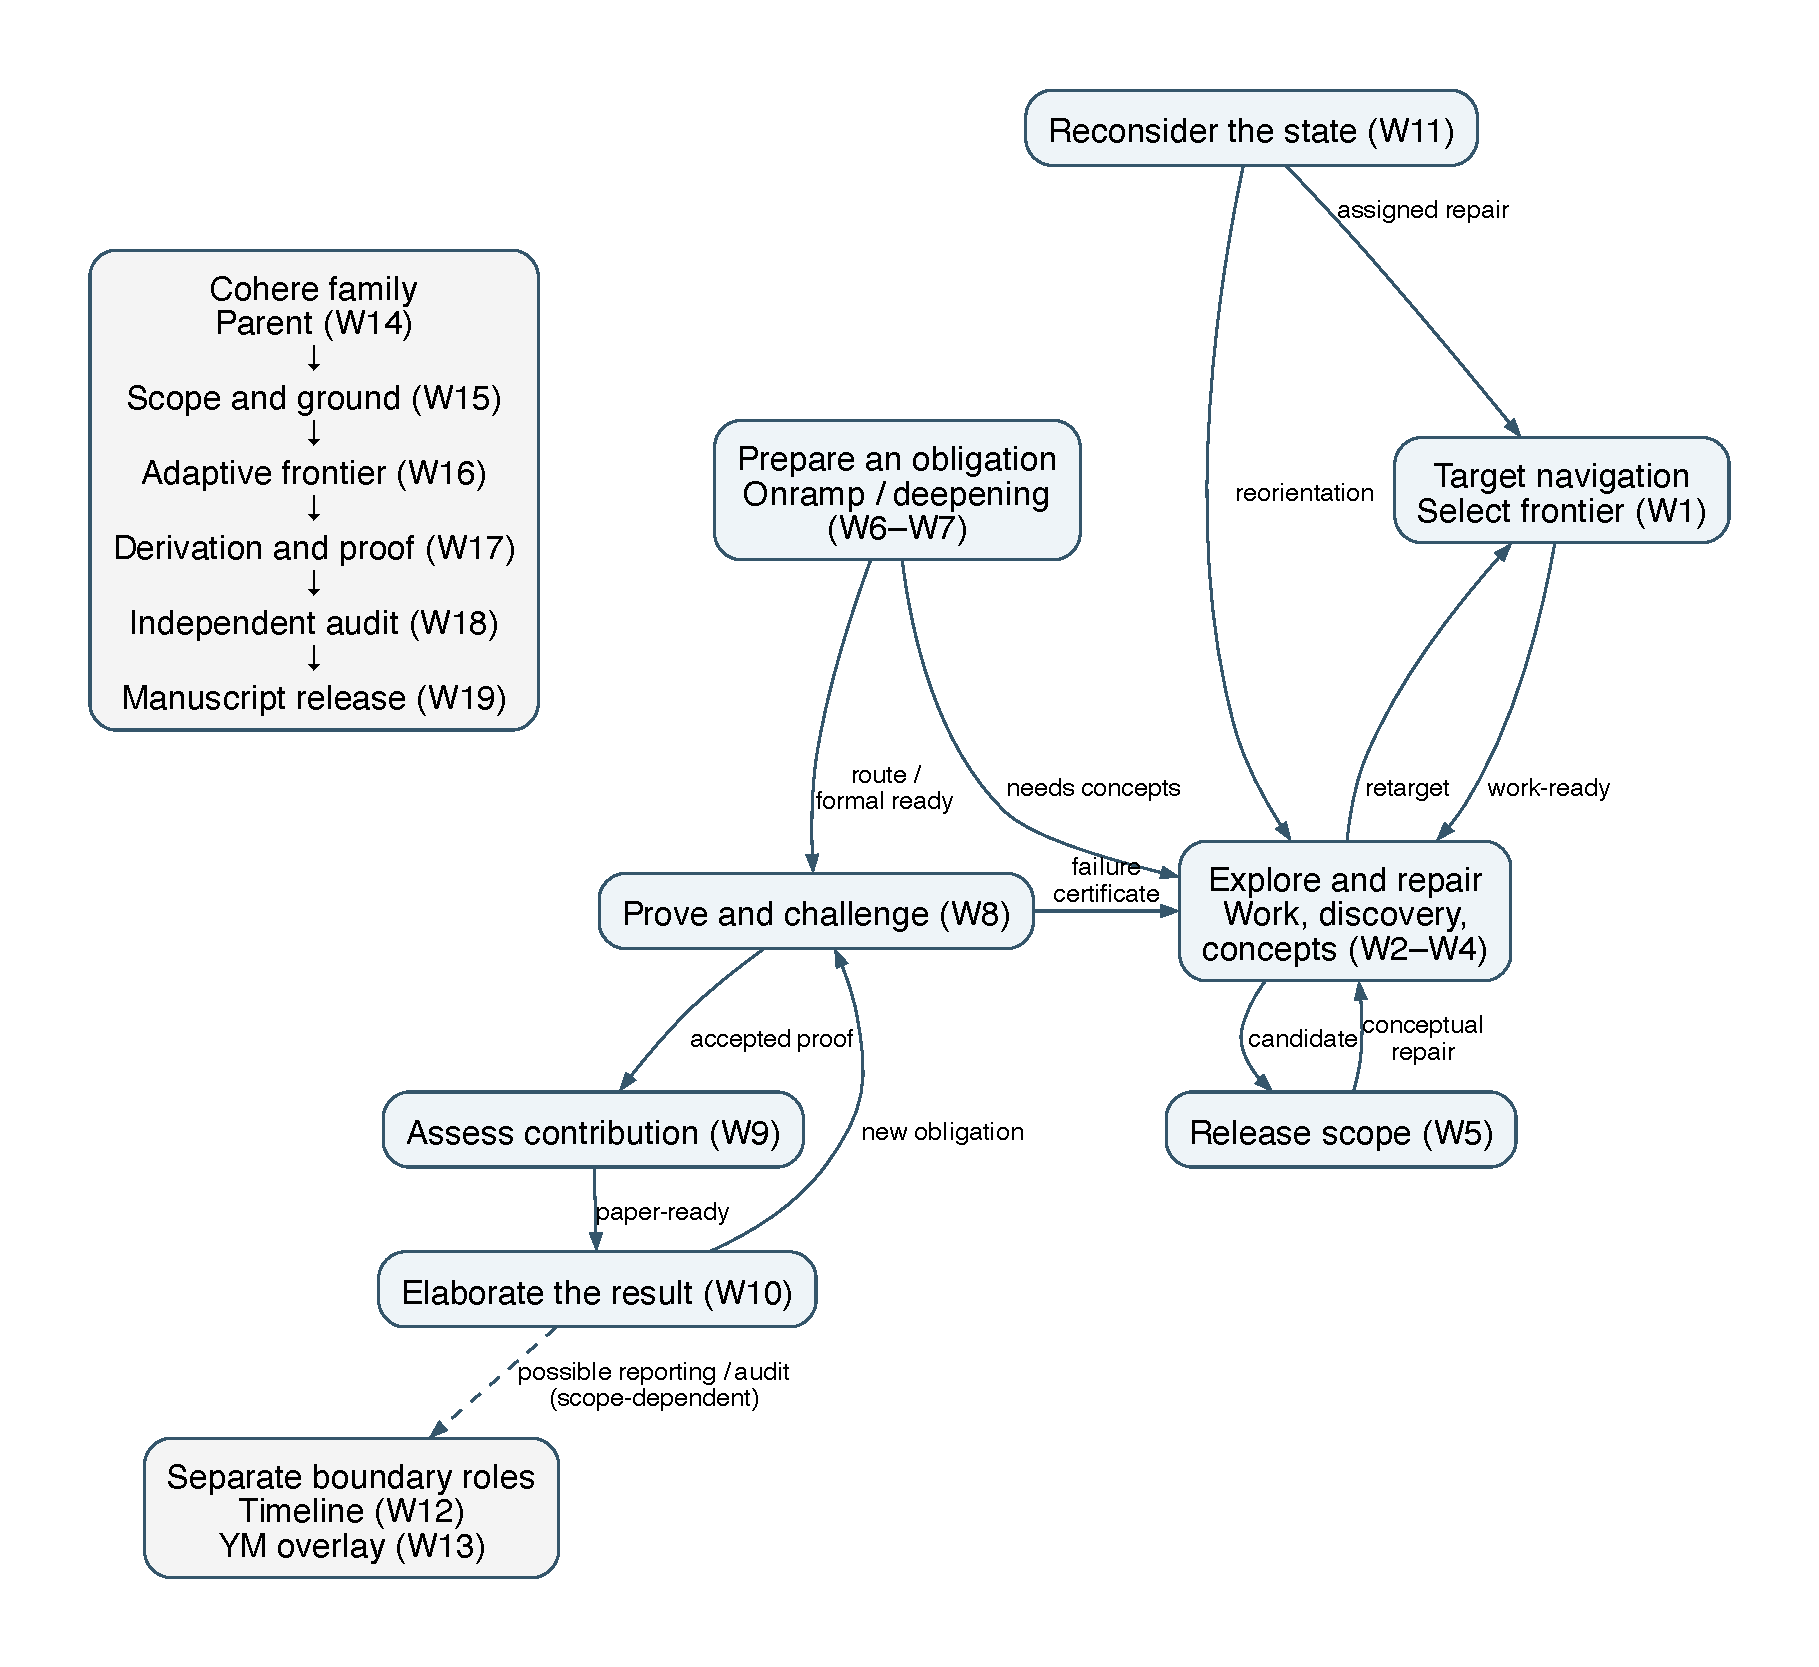
\includegraphics[width=\linewidth]{paper-workflow-representations/workflow-ecosystem.pdf}
\caption{A grouped map of research roles. Solid arrows summarize prescribed
routing between selected members of the grouped workflow families, not all
member-to-member connections or every declared edge; dashed arrows denote editorial
feedback or applicability, requiring an explicit handoff. The separate Cohere
box has declared internal subworkflow composition, but no general-discovery
entry edge is asserted. Exact workflow names and source qualifications appear
in Appendix~\ref{app:workflow-relationships}.}
\label{fig:workflow-ecosystem}
\end{figure}

\paragraph{Orient and explore.}
Target navigation identifies which unresolved obligation deserves the next
allocation. A focused abductive loop can address a bounded explanatory gap;
a discovery marathon coordinates a wider portfolio. Conceptual hypothesis
exploration and conceptual frontier deepening address failures of the inherited
representation and mature alternatives through reflection. Their contribution
is to make a better question or candidate available, with its protected
successes, objections and burdens. A diagnostic no-preference outcome returns
for revision; it does not itself authorize a preferred proof route.

\paragraph{Turn a mature question into support.}
The evidence-to-proof onramp develops a route from an evidence-bearing candidate;
theorem proof delivery addresses an exact theorem and its closure conditions.
These can become children of a conceptual programme when the programme has
produced the necessary question and the source gates permit the handoff.
A proof result answers its exact obligation. A failed transfer or unresolved
premise returns a blocker that can motivate route revision or conceptual
reconsideration, with the broader return connection made explicit by the caller.

\paragraph{Reconsider and consolidate.}
Deep review and reorientation examines the current reasoning state and can
produce a corrective agenda. Scientific contribution cultivation asks whether
a result has a defensible independent payoff; manuscript result elaboration
explicates its actual consequences and remaining limits. Release promotion
judges whether the relevant evidence and gates support a release disposition.
These activities have different acceptance conditions: a coherent exposition,
a worthwhile contribution, a proved theorem and a release decision are not
interchangeable achievements.

\paragraph{Keep special compositions and overlays in scope.}
Cohere is a separately declared parent workflow whose children scope and ground,
explore an adaptive frontier, derive and prove, independently audit, and prepare
manuscript release. Its structure supplies a concrete example of nested work,
but unresolved native producers remain projection gaps. The timeline-paper
workflow independently reports a bounded research history; it does not confer
proof authority. The Yang--Mills representational-dynamics overlay attaches
domain-specific representational checks to an applicable inquiry. Neither its
name nor its inclusion makes a result a Yang--Mills theorem. These boundary
roles should be attached only where their input and scope requirements fit.

Across these families, recursive goal records provide a common \emph{handoff
interpretation}: identify the parent question, the requested contribution, the
accepted evidence and the conditions for returning or stopping. They do not
supply missing executable wiring. A workflow can discharge a subgoal, create
new children, recommend another route, or return a reason to stop. The parent
retains responsibility for interpreting that outcome against the scientific
question that made the invocation worthwhile.
